\section*{Introduction}

The 21st century is an exciting time to be doing science. Specifcally, computational biosciences have taken a central role in today's world, starting from the Human Genome Project \citep{international2001initial}, unveiled at the turn of the century. Fast-forward  two decades: the complete sequence of a human genome  \citep{nurk2022complete} is unveiled. However, sequence is only one side of the coin, as the drivers of the most intricate cellular processes are structures of biomolecules. Complex biophysical processes govern how the genome is regulated and transcribed \citep{lambert2018human}, and during these processes the biological reality of the genome is often far from the standard B-DNA structure discovered more than 70 years ago \citep{watson1953}. A beautiful reminder of this is the modeled complex of the human interferon beta enhanceosome \citep{panne2007atomic}, shown in \blue{Fig. \ref{fig:mmc2}}. The structure displays remarkably intricate shape, a regulatory DNA segment occupies, to serve as binding site for a plethora of eukaryotic transcription factors. This reality has been demonstrated \citep{rohs2009role} to be present in a broad scale across the structures deposited on the PDB \citep{berman2000protein}. Inspired by this fact, my primary focus has been deciphering protein-DNA interaction with data driven deep learning methods. I present, in chapter 1,
my work on the segmentation of protein surfaces into nucleic acid binding and non-binding regions. This chapter describes a graph neural network layer, which enables smooth prediction of binding site labels on the protein surface. We start from a model of nucleic acid binding site
prediction (PNAbind) developed in the Rohs lab and improve upon it by designing a neural network layer using mean field
VI over a continuous Conditional Random Field model, which makes the predicted binding sites smoother while improving upon prediction metrics. We also design a smoothness metric addressing the label imbalance problem associated with the task.
In Chapter 2, I describe DeepPBS (Deep predictor of binding specificity), the first of its kind geometric deep learning method developed to predict DNA binding specificity of proteins based on a given protein-DNA complex. DeepPBS acts as a bridge between structure determining (which shows mechanism but not sequence diversity) and specificity determining experiments (which reflects sequences diversity but not mechanism). DeepPBS is applicable on experimentally determined, simulated, predicted or designed complexes, resulting in a broad impact in the domain.

In chapter 3, we design and showcase the RNAscape algorithm and webserver, a geometric mapping method of RNA 3D structures to 2D, which attempts to preserve the three dimensional topology (unlike common secondary structure based visualization methods). RNAscape significantly improves over existing competitors in terms of the mapping quality, visualization and customisability.
\begin{center}
    \begin{figure}[H]
    \makebox[\textwidth]{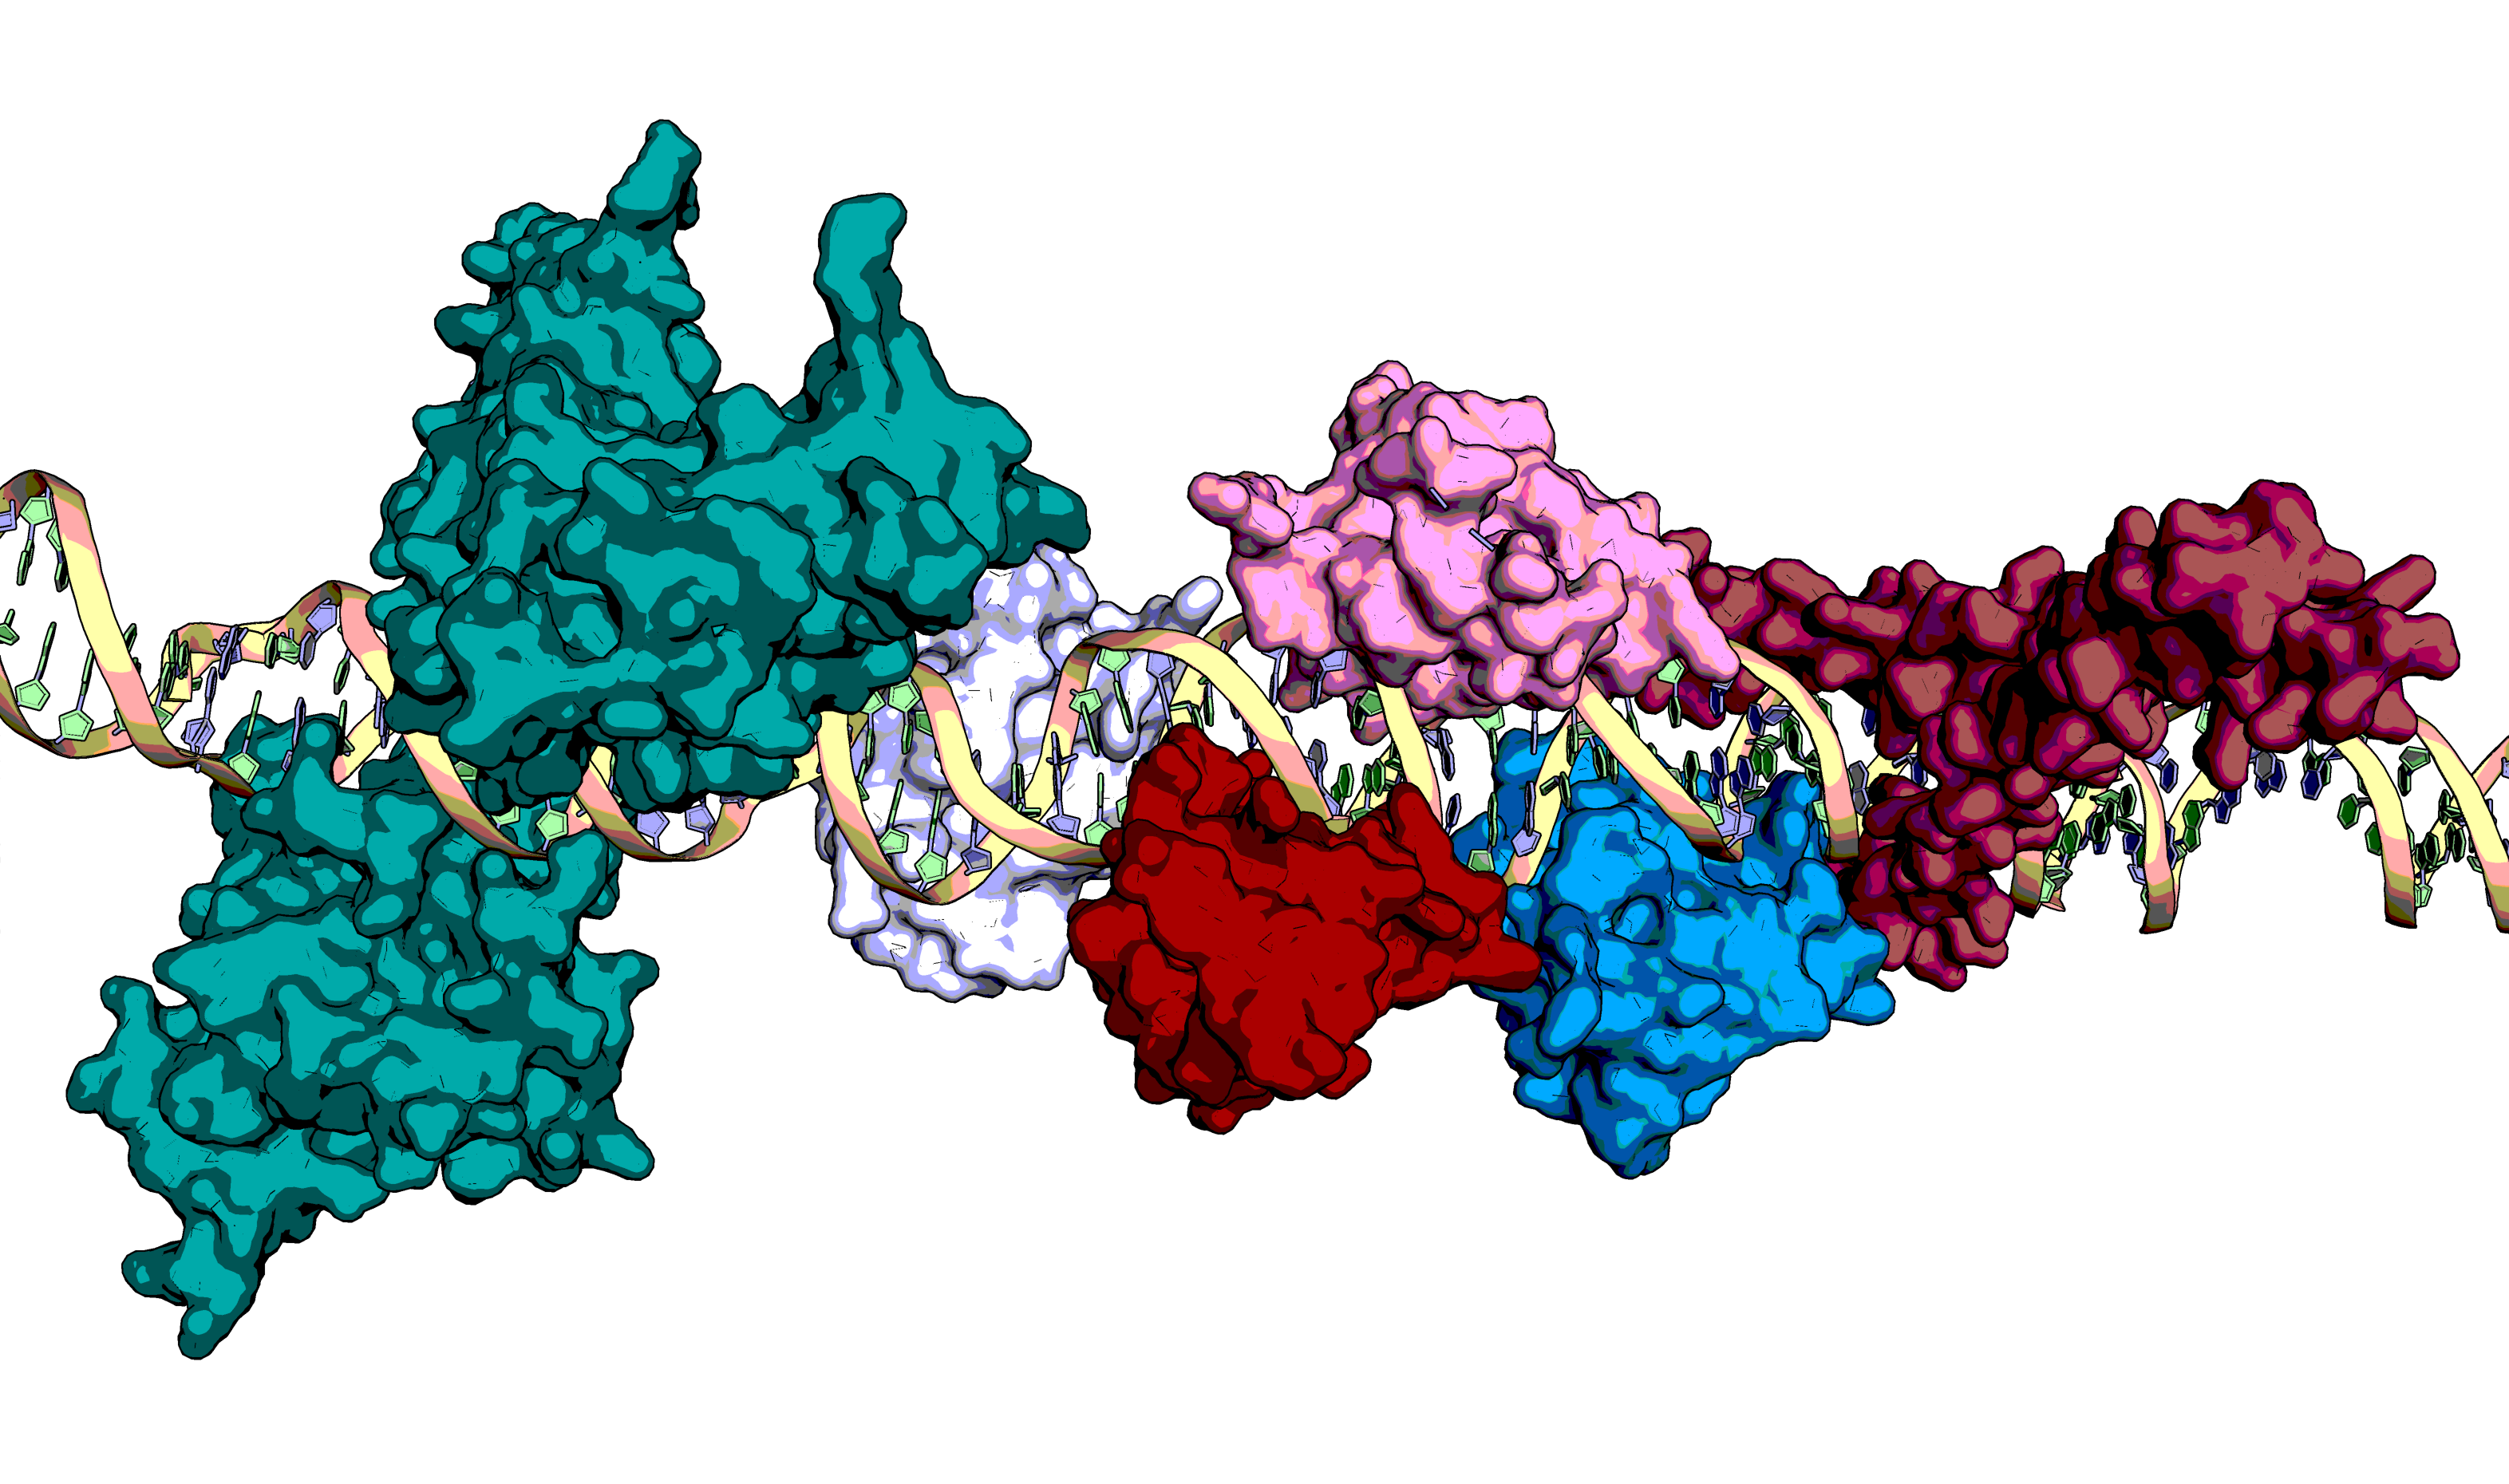
\includegraphics[width=0.8\textwidth]{./main/mmc2.png}}
 % archetecture.png: 1149x508 px, 72dpi, 40.53x17.92 cm, bb=0 0 1149 508
        \caption[Structure of the human interferon-beta enhanceosome]{\textbf{ Structure of the human interferon-beta enhanceosome} as modeled and published by \citet{panne2007atomic}. The protein chains are shown in a surface representation, one color for each unique monomer. DNA backbone is shown as a ribbon (wheat color). AT pairs are shown in light green while GC pairs are shown in lightblue. The view was chosen to emphasize the intricate DNA shape observed in the complex. The DNA has been extended slightly on both ends.}
  \label{fig:mmc2}
\end{figure}
\end{center}
Chapter 4 describes an updated DNAproDB database, which was originally implemented by Jared Sagendorf. Through this update we
introduce both technical advances and an expansion of features included in the analysis.
DNAproDB is now automatically updated weekly with newly released structures and thereby will
remain up to date as new DNA–protein structures are solved. We also include much larger
complexes, expand external annotations and upload/download formats, and improve the user
experience through a re-organization of the web interface and more visualization options and
controls. We added the annotation of water-mediated hydrogen bonds as a new feature.
At the same time we recognized lack of a comprehensive analysis and exploration tool for RNA/protein-RNA structures. Being inspired from RNAscape and DNAproDB, we developed RNAproDB, which is described in Chapter 5. RNAproDB is a modern highly interactive structure exploration tool tailored for the complexity and structural variance of RNA structures. This is achieved by intricate interplay of a 3D viewer, interface explorer, sequence viewer, secondary structure selector and tabular data:  making it the most versatile tool for analyzing and exploring protien-NA complexes. With the advent of complex structure prediction methods like AlphaFold3, we expect RNAproDB to serve a crucial role in analyzing predicted structures and advance the understanding of cellular biology.
In chapter 6, I present an autoencoder model applicable on gene expression time-series data, to learn a regularized latent
space representation and a generative process. RVAgene is primarily a visualization tool suitable for biological
knowledge discovery, while also being suitable for de novo data generation, denoising and a more
efficient alternative to hierarchical Gaussian process based methods to cluster such data. We
analyze one synthetic and two real datasets and demonstrate various properties and aspects of the
model and its potential for unsupervised discovery.  In particular, RVAgene identifies new programs of
shared gene regulation of \textit{Lox} family genes in response to kidney injury. We conclude this thesis by discussing current state of the field of structural biology of protein-nucleic acid complexes and future possibilities.
